% Rx32 block diagram.
\documentclass[tikz,border=0pt]{standalone}
\usepackage{fontspec}
\IfFontExistsTF{Lato}
  {\setsansfont{Lato}[BoldFont={Lato Semibold}]}
  {\setsansfont{TeX Gyre Heros}}
\IfFontExistsTF{Ubuntu Mono}
  {\setmonofont{Ubuntu Mono}}
  {\setmonofont{Latin Modern Mono}}
\renewcommand\familydefault{\sfdefault}
\usetikzlibrary{arrows.meta,calc}

\definecolor{paper}{HTML}{FFFFFF}
\definecolor{ink}{HTML}{23272E}
\definecolor{mute}{HTML}{6B7380}
\definecolor{ctl}{HTML}{98A0AA}
\definecolor{bar}{HTML}{D3D8DE}
\definecolor{t0}{HTML}{4682CC}
\definecolor{t1}{HTML}{00A396}
\definecolor{t2}{HTML}{E4A339}
\definecolor{t3}{HTML}{E16A3E}
\definecolor{t4}{HTML}{B25196}

\newcommand\fstage{\fontsize{6.5}{7}\selectfont\bfseries\addfontfeatures{LetterSpace=10}}
\newcommand\ftitle{\fontsize{7}{8}\selectfont\bfseries}
\newcommand\fsub{\fontsize{5.5}{6.5}\selectfont\color{mute}}
\newcommand\fsig{\fontsize{5.5}{6}\selectfont\ttfamily\color{mute}}
\newcommand\thr[1]{\tikz[baseline=-0.55ex]\fill[#1] (0,0) circle (1.25pt);\,}

\pgfdeclarelayer{paper}\pgfdeclarelayer{ctl}\pgfdeclarelayer{bridge}\pgfdeclarelayer{data}
\pgfsetlayers{paper,ctl,bridge,data,main}

\begin{document}
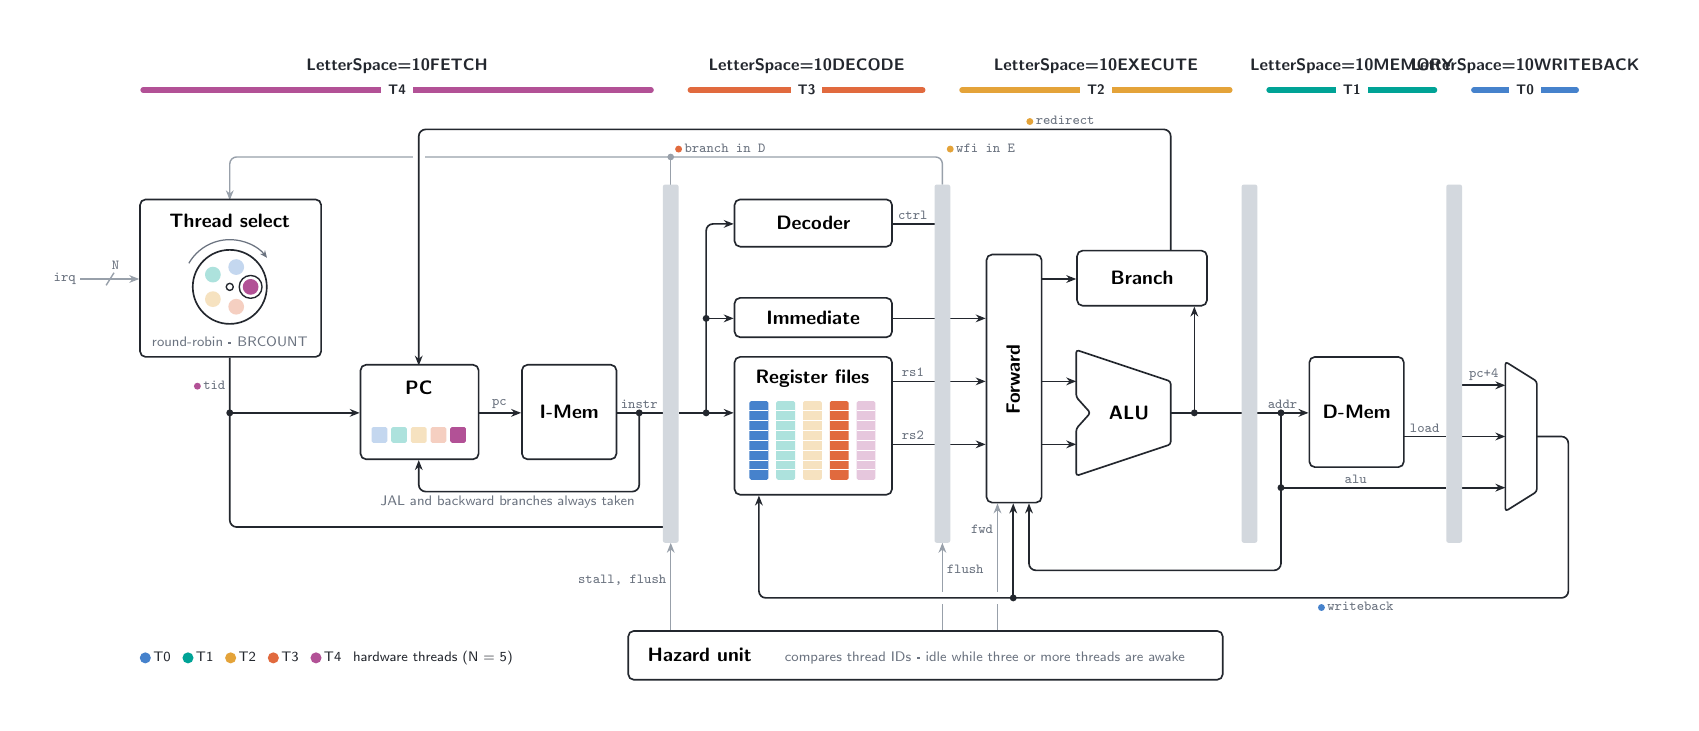
\begin{tikzpicture}[
    line join=round,
    block/.style={draw=ink, line width=0.6pt, fill=paper, rounded corners=2pt},
    w/.style={draw=ink, line width=0.6pt, rounded corners=2.5pt},
    c/.style={draw=ctl, line width=0.5pt, rounded corners=2.5pt},
    >={Stealth[length=3.6pt,width=2.8pt]},
    dot/.style={circle, fill=ink, inner sep=0pt, minimum size=2.5pt},
    cdot/.style={circle, fill=ctl, inner sep=0pt, minimum size=2.4pt},
    sig/.style={font=\fsig, inner sep=1.4pt},
  ]

\def\yS{3.6}                                   % datapath spine
\def\yBb{1.95}  \def\yBt{6.5}                  % pipeline register extent
\def\yStat{6.85} \def\yRed{7.2}                % lanes back to fetch
\def\yFM{1.6}   \def\yWB{1.25}                 % forward / writeback lanes
\def\xFD{6.75} \def\xDE{10.2} \def\xEM{14.1} \def\xMW{16.7}
\def\h{0.1}                                    % half a pipeline register

\newcommand\bridge[2]{\begin{pgfonlayer}{bridge}
  \fill[paper] ($(#1)+(#2)$) rectangle ($(#1)-(#2)$);\end{pgfonlayer}}
\newcommand\blk[6]{%
  \node[block, anchor=south west, minimum width=#4cm, minimum height=#5cm] (#1) at (#2,#3) {};
  \node[font=\ftitle] at (#1.center) {#6};}

\foreach \name/\xa/\xb/\t in {FETCH/0/6.55/4, DECODE/6.95/10.0/3,
    EXECUTE/10.4/13.9/2, MEMORY/14.3/16.5/1, WRITEBACK/16.9/18.3/0} {
  \node[font=\fstage, text=ink] at ({(\xa+\xb)/2}, 8.0) {\name};
  \draw[t\t, line width=2pt, line cap=round] (\xa+0.05, 7.7) -- (\xb-0.05, 7.7);
  \node[fill=paper, inner xsep=2.5pt, inner ysep=0.5pt, font=\fontsize{5.5}{6}\selectfont\bfseries, text=ink]
    at ({(\xa+\xb)/2}, 7.7) {T\t};
}

\foreach \x in {\xFD,\xDE,\xEM,\xMW}
  \fill[bar, rounded corners=0.8pt] (\x-\h,\yBb) rectangle (\x+\h,\yBt);

\node[block, anchor=south west, minimum width=2.3cm, minimum height=2cm] (ts) at (0,4.3) {};
\node[font=\ftitle] at (1.15,6.04) {Thread select};
\node[font=\fsub] at (1.15,4.5) {round-robin · BRCOUNT};
\begin{scope}[shift={(1.15,5.2)}]
  \draw[ink, line width=0.6pt] (0,0) circle (0.47);
  \foreach \t/\a in {0/72, 1/144, 2/216, 3/288}
    \fill[t\t!32!paper] (\a:0.265) circle (0.1);
  \fill[t4] (0:0.265) circle (0.1);
  \draw[ink, line width=0.5pt] (0:0.265) circle (0.145);
  \draw[ink, line width=0.5pt, fill=paper] (0,0) circle (0.045);
  \draw[mute, line width=0.45pt, ->, >={Stealth[length=2.6pt,width=2.2pt]}]
    (150:0.6) arc[start angle=150, end angle=38, radius=0.6];
\end{scope}

\node[block, anchor=south west, minimum width=1.5cm, minimum height=1.2cm] (pc) at (2.8,3.0) {};
\node[font=\ftitle] at (3.55,3.92) {PC};
\foreach \t/\k in {0/32,1/32,2/32,3/32,4/100}
  \fill[rounded corners=0.6pt, t\t!\k!paper] (2.95+\t*0.25,3.22) rectangle ++(0.2,0.2);

\blk{im}{4.85}{3.0}{1.2}{1.2}{I-Mem}

\blk{dec}{7.55}{5.7}{2}{0.6}{Decoder}
\blk{imm}{7.55}{4.55}{2}{0.5}{Immediate}
\node[block, anchor=south west, minimum width=2cm, minimum height=1.75cm] (rf) at (7.55,2.55) {};
\node[font=\ftitle] at (8.55,4.03) {Register files};
\foreach \t/\k in {0/100,1/32,2/32,3/100,4/32} {
  \fill[rounded corners=0.6pt, t\t!\k!paper] (7.75+\t*0.34,2.75) rectangle ++(0.24,1.0);
  \foreach \r in {1,...,7}
    \draw[paper, line width=0.35pt] (7.75+\t*0.34,2.75+\r*0.125) -- ++(0.24,0);
}

\node[block, anchor=south west, minimum width=0.7cm, minimum height=3.15cm] (fw) at (10.75,2.45) {};
\node[font=\ftitle, rotate=90] at (11.1,4.02) {Forward};
\blk{br}{11.9}{4.95}{1.65}{0.7}{Branch}
\draw[block, rounded corners=1pt] (11.9,2.8) -- (13.1,3.2) -- (13.1,4.0) -- (11.9,4.4)
  -- (11.9,3.8) -- (12.08,3.6) -- (11.9,3.4) -- cycle;
\node[font=\ftitle] at (12.57,\yS) {ALU};

\blk{dm}{14.85}{2.9}{1.2}{1.4}{D-Mem}
\draw[block, rounded corners=1pt] (17.35,2.35) -- (17.75,2.6) -- (17.75,4.0) -- (17.35,4.25) -- cycle;

\node[block, anchor=south west, minimum width=7.55cm, minimum height=0.62cm] (hz) at (6.2,0.2) {};
\node[anchor=west, inner sep=0pt] (hzt) at (6.45,0.51)
  {{\ftitle Hazard unit}\hspace{1.2em}{\fsub compares thread IDs · idle while three or more threads are awake}};

\node[anchor=base west, inner sep=0pt, font=\fsub] at (hzt.base -| 0,0) {%
  \foreach \t in {0,...,4}{\tikz[baseline=-0.6ex]\fill[t\t] (0,0) circle (2pt);\,{\color{ink}T\t}\hspace{0.8em}}%
  {\color{ink}hardware threads (N = 5)}};

\begin{pgfonlayer}{data}
  % Fetch.
  \draw[w] (1.15,4.3) -- (1.15,2.15) -- (\xFD-\h,2.15);
  \draw[w,->] (1.15,\yS) -- (2.8,\yS);
  \draw[w,->] (4.3,\yS) -- (4.85,\yS);
  \draw[w] (6.05,\yS) -- (\xFD-\h,\yS);
  \draw[w,->] (6.35,\yS) -- (6.35,2.6) -- (3.55,2.6) -- (3.55,3.0);   % predecode
  % Decode.
  \draw[w,->] (\xFD+\h,\yS) -- (7.55,\yS);
  \draw[w,->] (7.2,\yS) -- (7.2,6.0) -- (7.55,6.0);
  \draw[w,->] (7.2,4.8) -- (7.55,4.8);
  \foreach \y in {6.0,4.8,4.0,3.2} \draw[w] (9.55,\y) -- (\xDE-\h,\y);
  % Execute.
  \foreach \y in {4.8,4.0,3.2} \draw[w,->] (\xDE+\h,\y) -- (10.75,\y);
  \foreach \y in {5.3,4.0,3.2} \draw[w,->] (11.45,\y) -- (11.9,\y);
  \draw[w] (13.1,\yS) -- (\xEM-\h,\yS);
  \draw[w,->] (13.4,\yS) -- (13.4,4.95);
  % Memory.
  \draw[w,->] (\xEM+\h,\yS) -- (14.85,\yS);
  \draw[w] (14.5,2.65) -- (\xMW-\h,2.65);
  \draw[w] (16.05,3.3) -- (\xMW-\h,3.3);
  % Writeback.
  \foreach \y in {3.95,3.3,2.65} \draw[w,->] (\xMW+\h,\y) -- (17.35,\y);
  % Redirect back to fetch.
  \draw[w,->] (13.1,5.65) -- (13.1,\yRed) -- (3.55,\yRed) -- (3.55,4.2);
  % Writeback and forwarding.
  \draw[w,->] (17.75,3.3) -- (18.15,3.3) -- (18.15,\yWB) -- (7.87,\yWB) -- (7.87,2.55);
  \draw[w,->] (11.1,\yWB) -- (11.1,2.45);
  \draw[w,->] (14.5,\yS) -- (14.5,\yFM) -- (11.3,\yFM) -- (11.3,2.45);
\end{pgfonlayer}
\foreach \p in {(1.15,\yS),(7.2,\yS),(7.2,4.8),(13.4,\yS),(14.5,\yS),(14.5,2.65),(11.1,\yWB),(6.35,\yS)}
  \node[dot] at \p {};

\begin{pgfonlayer}{ctl}
  \draw[c,->] (-0.75,5.3) -- (0,5.3);
  \draw[c] (-0.42,5.22) -- (-0.32,5.38);
  \draw[c,->] (\xDE,\yBt) -- (\xDE,\yStat) -- (1.15,\yStat) -- (1.15,6.3);
  \draw[c] (\xFD,\yBt) -- (\xFD,\yStat);
  \draw[c,->] (\xFD,0.82) -- (\xFD,\yBb);
  \draw[c,->] (\xDE,0.82) -- (\xDE,\yBb);
  \draw[c,->] (10.9,0.82) -- (10.9,2.45);
\end{pgfonlayer}
\node[cdot] at (\xFD,\yStat) {};
\bridge{3.55,\yStat}{0.075,0.09}
\bridge{\xDE,\yWB}{0.09,0.075}
\bridge{10.9,\yWB}{0.09,0.075}

\node[sig, anchor=east] at (-0.75,5.3) {irq};
\node[sig, anchor=south, inner sep=0.8pt] at (-0.3,5.38) {N};
\node[sig, anchor=east] at (1.15,3.95) {\thr{t4}tid};
\node[sig, anchor=south] at (4.575,\yS) {pc};
\node[sig, anchor=south] at (6.35,\yS) {instr};
\node[sig, anchor=south] at (9.825,6.0) {ctrl};
\node[sig, anchor=south] at (9.825,4.0) {rs1};
\node[sig, anchor=south] at (9.825,3.2) {rs2};
\node[sig, anchor=south west] at (\xFD,\yStat) {\thr{t3}branch in D};
\node[sig, anchor=south west] at (\xDE,\yStat) {\thr{t2}wfi in E};
\node[sig, anchor=south] at (11.7,\yRed) {\thr{t2}redirect};
\node[sig, anchor=south] at (14.52,\yS) {addr};
\node[sig, anchor=south] at (16.325,3.3) {load};
\node[sig, anchor=south] at (15.45,2.65) {alu};
\node[sig, anchor=south] at (17.075,3.95) {pc+4};
\node[sig, anchor=north] at (15.45,\yWB) {\thr{t0}writeback};
\node[sig, anchor=east] at (\xFD,1.48) {stall, flush};
\node[font=\fsub, anchor=north east, inner sep=1.4pt] at (6.35,2.6) {JAL and backward branches always taken};
\node[sig, anchor=west] at (\xDE,1.62) {flush};
\node[sig, anchor=east] at (10.9,2.12) {fwd};

\begin{pgfonlayer}{paper}
  \fill[paper] ([shift={(-8pt,-8pt)}]current bounding box.south west)
    rectangle ([shift={(8pt,8pt)}]current bounding box.north east);
\end{pgfonlayer}
\end{tikzpicture}
\end{document}
